\documentclass[11pt,a4paper]{article}
\usepackage[margin=24mm]{geometry}
\usepackage{amsmath,graphicx,booktabs,float,hyperref}
\usepackage{tikz}
\usetikzlibrary{arrows.meta,positioning}
\usepackage{parskip}
\hypersetup{colorlinks=true,urlcolor=blue}
\title{12-Lead ECG Forecasting with LSTM and CNN-LSTM\\\large Revised Assignment 4}
\author{Omar Faruk \and Md Mustak Talukder \and Md. Forman Ullah Sajib \and Ehsan Robbany Chowdhury}
\date{Instructor: Dr. Fatima Sajid Butt\\Winter Semester 2026/27}
\begin{document}
\maketitle
\begin{abstract}
We compare LSTM and CNN-LSTM models for forecasting the last three seconds of a 12-lead ECG from its first seven seconds. We use the full available training and validation folds of PTB-XL and train each model for 120 epochs, with and without filtering of the observed signal. On the validation fold, the CNN-LSTM achieved lower error than the LSTM in both settings. Filtering slightly reduced LSTM error but increased CNN-LSTM error. These are validation results; the reserved test fold has not been evaluated.
\end{abstract}
\section{Data, task and folds}
PTB-XL version 1.0.3 contains 21,799 ten-second ECG recordings from 18,869 patients \cite{ptbxl}. We use its 100 Hz recordings, with 1,000 samples per lead. The twelve leads are I, II, III, aVR, aVL, aVF, V1, V2, V3, V4, V5 and V6. The first 700 samples (7 seconds) are the input; the remaining 300 samples (3 seconds) are the prediction target. Each recording contributes one window. This predicts a later part of the same recording.

The dataset provides ten patient-stratified folds. We use folds 1--8 for training, fold 9 for validation and fold 10 as a reserved test set. A patient's records remain in one fold, so patients do not overlap between these groups. This is one fixed split, not ten rounds of cross-validation. Validation selects the best epoch; fold 10 has not been used to calculate the results in this report.
\begin{center}
\begin{tabular}{llrr}\toprule
Purpose & Folds & ECG records & Patients \\\midrule
Training & 1--8 & 17,418 & 15,023 \\
Validation & 9 & 2,183 & 1,942 \\
Reserved test & 10 & 2,198 & 1,904 \\\bottomrule
\end{tabular}
\end{center}
The previous submission described an expanded cohort of 4,500 training patients. The present training set uses 15,023 patients. The previous report used a 5-second input and 3-second forecast; this report uses 7 seconds and 3 seconds, so its scores are not a controlled comparison of dataset size alone.
\section{Preprocessing}
We compare two input settings. In the \textbf{unfiltered} setting, the recorded input is used without additional filtering. In the \textbf{filtered} setting, a causal Butterworth bandpass filter from 0.5 to 40 Hz is applied to the observed seven seconds only. The filter is intended to reduce slow baseline changes and high-frequency noise. It can also change the shape and timing of the waveform.

Both settings use the same per-lead standardization, calculated from unfiltered training inputs only:
\begin{equation}
 z_{t,l}=\frac{x_{t,l}-\mu_l}{\sigma_l}.
\end{equation}
Here $x_{t,l}$ is the voltage at time $t$ in lead $l$, and $\mu_l$ and $\sigma_l$ are the training-input mean and standard deviation for that lead. For the filtered setting, $x_{t,l}$ in this equation is the filtered input; the same training statistics are used in both settings. The future target remains the original unfiltered signal. Predictions are converted back to millivolts before evaluation. Therefore, the comparison measures the effect of filtering in addition to standardization, rather than a comparison against completely unprocessed input.
\section{Model architectures}
\subsection{LSTM}
A long short-term memory (LSTM) network reads the 12 lead values at each time step in order. Its cell state carries information through time. Gates control what is retained, added and passed to the output. At time $t$ the standard LSTM equations are
\begin{align}
 f_t&=\sigma(W_f[x_t,h_{t-1}]+b_f), & i_t&=\sigma(W_i[x_t,h_{t-1}]+b_i),\\
 \widetilde c_t&=\tanh(W_c[x_t,h_{t-1}]+b_c), & c_t&=f_t\odot c_{t-1}+i_t\odot\widetilde c_t,\\
 o_t&=\sigma(W_o[x_t,h_{t-1}]+b_o), & h_t&=o_t\odot\tanh(c_t).
\end{align}
Here $x_t$ is the current input, $h_{t-1}$ the previous hidden state and $c_{t-1}$ the previous cell state. The forget gate $f_t$ controls retained memory; the input gate $i_t$ controls the candidate information $\widetilde c_t$ added to it; the output gate $o_t$ controls the hidden state $h_t$. The weights $W$ and biases $b$ are learned; $\sigma$ gives values between zero and one, $\tanh$ gives values between $-1$ and $1$, and $\odot$ denotes element-wise multiplication.

In the implementation, an input recording has 700 time steps and 12 values at each step. A batch of $B$ recordings therefore has shape $B\times700\times12$. One LSTM layer with 64 hidden units reads the 700 vectors sequentially. At each step, the same learned gate weights are reused, while the cell and hidden states change. After the last observed step, its 64-value hidden state summarizes the input and is passed to the forecast head.

The head first maps the 64 values to 128 values, applies ReLU and dropout with probability 0.2 during training, and then maps the result to $300\times12=3{,}600$ output values. Dropout temporarily sets a random fraction of head activations to zero during training; it is disabled when evaluating the model. The output is reshaped to $B\times300\times12$. Thus, the network predicts all future points together from the final hidden state, rather than feeding each predicted point back into the LSTM. The model uses ECG values only; no age, sex or diagnosis inputs are included in these four runs.

\textbf{Data flow:} 700 observed 12-lead samples $\rightarrow$ LSTM (64 hidden units) $\rightarrow$ dense layer (128 units) $\rightarrow$ 3,600 outputs $\rightarrow$ 300 predicted samples for each lead.
\begin{figure}[H]
\centering
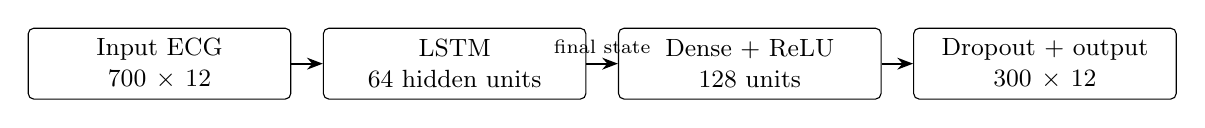
\begin{tikzpicture}[
  node distance=4mm,
  block/.style={draw, rounded corners=2pt, align=center, minimum height=9mm, text width=31mm, font=\small},
  arrow/.style={-{Stealth[length=2mm]}, thick}
]
\node[block] (input) {Input ECG\\$700\times12$};
\node[block, right=of input] (lstm) {LSTM\\64 hidden units};
\node[block, right=of lstm] (dense) {Dense + ReLU\\128 units};
\node[block, right=of dense] (out) {Dropout + output\\$300\times12$};
\draw[arrow] (input) -- (lstm);
\draw[arrow] (lstm) -- node[above,font=\scriptsize] {final state} (dense);
\draw[arrow] (dense) -- (out);
\end{tikzpicture}
\caption{LSTM architecture. The final hidden state is used to predict all future lead values together.}
\label{fig:lstm_arch}
\end{figure}

\subsection{CNN-LSTM}
The CNN-LSTM combines a convolutional feature extractor with an LSTM. It first applies one-dimensional convolutions along time to extract local patterns from the 12 leads. For a convolution output channel $k$ a simplified expression is
\begin{equation}
 a_{t,k}=\operatorname{ReLU}\!\left(b_k+\sum_l\sum_j w_{k,l,j}x_{t+j,l}\right).
\end{equation}
Here $w_{k,l,j}$ are learned filter weights, $b_k$ is a bias, and ReLU replaces negative values with zero. The index $l$ runs over input channels and $j$ over nearby time positions. A filter moves along the observed signal, using the same weights at different positions to detect a learned local pattern.

The input again has 700 time steps and 12 leads. The first convolution uses 32 filters of width 7; each filter combines information from all 12 input leads over seven neighboring samples. Padding keeps the sequence length at 700. ReLU is then applied. A second convolution uses 64 filters of width 5, again with padding and ReLU, producing 64 features at each of the 700 positions. Average pooling then averages each pair of neighboring positions, reducing the length to 350. The 64 features at each of these 350 positions form the sequence passed to one LSTM layer with 64 hidden units.

The last LSTM hidden state enters the same type of forecast head as in the LSTM model: a 128-unit dense layer, ReLU, dropout of 0.2 during training, and a 3,600-value output layer reshaped to 300 samples for each of the 12 leads. The convolution and LSTM weights are learned together during training. Pooling reduces the number of recurrent steps, but averaging can also smooth sharp features.

\textbf{Data flow:} 700 observed 12-lead samples $\rightarrow$ convolution (32 filters) $\rightarrow$ convolution (64 filters) $\rightarrow$ pooling (350 steps) $\rightarrow$ LSTM (64 units) $\rightarrow$ dense head $\rightarrow$ 300 predicted samples for each lead.

The key difference is the input to the recurrent layer: the LSTM model reads the standardized lead values directly, whereas CNN-LSTM first transforms them into local features. Both models use the full observed window and predict the same three-second future.
\begin{figure}[H]
\centering
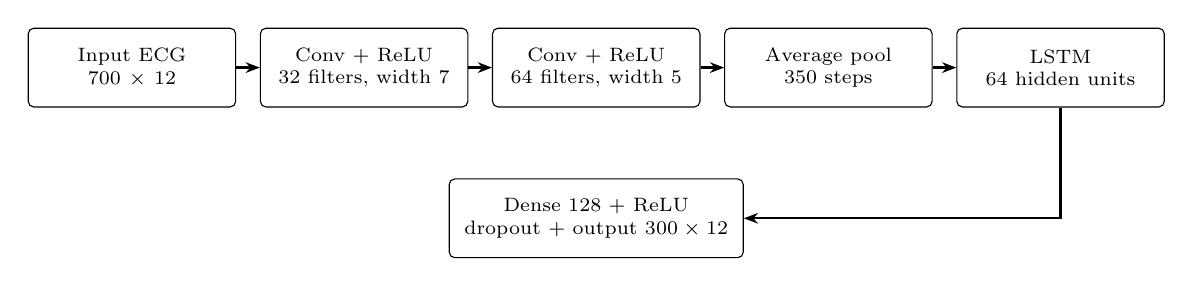
\begin{tikzpicture}[
  node distance=3mm,
  block/.style={draw, rounded corners=2pt, align=center, minimum height=10mm, text width=24mm, font=\scriptsize},
  arrow/.style={-{Stealth[length=1.8mm]}, thick}
]
\node[block] (input) {Input ECG\\$700\times12$};
\node[block, right=of input] (c1) {Conv + ReLU\\32 filters, width 7};
\node[block, right=of c1] (c2) {Conv + ReLU\\64 filters, width 5};
\node[block, right=of c2] (pool) {Average pool\\350 steps};
\node[block, right=of pool] (lstm) {LSTM\\64 hidden units};
\draw[arrow] (input) -- (c1);
\draw[arrow] (c1) -- (c2);
\draw[arrow] (c2) -- (pool);
\draw[arrow] (pool) -- (lstm);
\node[block, below=9mm of c2, text width=35mm] (head) {Dense 128 + ReLU\\dropout + output $300\times12$};
\draw[arrow] (lstm.south) |- (head.east);
\end{tikzpicture}
\caption{CNN-LSTM architecture. Convolutions extract local features; the LSTM summarizes the pooled feature sequence for forecasting.}
\label{fig:cnn_arch}
\end{figure}

\section{Training and evaluation}
Four models were trained: each architecture with unfiltered and filtered inputs. All use the same train and validation records, a batch size of 64, AdamW optimization and 120 epochs. The LSTM learning rate was 0.0005 and the CNN-LSTM learning rate was 0.001. The model saved for reporting is the epoch with the lowest validation patient-average MAE. Training uses mean squared error on standardized targets; reporting uses original millivolts.

For actual voltages $y_i$ and predictions $\widehat y_i$, over $N$ forecast values, the metrics are
\begin{equation}
 \mathrm{MAE}=\frac{1}{N}\sum_{i=1}^{N}|\widehat y_i-y_i|,
 \qquad
 \mathrm{RMSE}=\sqrt{\frac{1}{N}\sum_{i=1}^{N}(\widehat y_i-y_i)^2}.
\end{equation}
Both are in mV and smaller is better. MAE is the average absolute voltage error. RMSE squares the errors before averaging, so large errors have more influence. \textbf{RMSE is applicable to LSTM}: it measures numerical prediction error and can be used for any model producing continuous values, including CNN-LSTM. Here the values aggregate the 300 predicted samples, 12 leads and all validation records.
\section{Results and comparison}
\begin{table}[H]\centering
\caption{Validation performance after 120 training epochs. Best epoch is selected using patient-average validation MAE.}
\begin{tabular}{llrrr}\toprule
Model & Input & MAE (mV) & RMSE (mV) & Best epoch \\\midrule
LSTM & Unfiltered & 0.1117 & 0.2344 & 29 \\
LSTM & Filtered & 0.1108 & 0.2312 & 99 \\
CNN-LSTM & Unfiltered & 0.1058 & 0.2266 & 116 \\
CNN-LSTM & Filtered & 0.1094 & 0.2278 & 43 \\\bottomrule
\end{tabular}
\end{table}
For LSTM, filtering reduced MAE from 0.1117 to 0.1108 mV and RMSE from 0.2344 to 0.2312 mV. For CNN-LSTM, filtering increased MAE from 0.1058 to 0.1094 mV and RMSE from 0.2266 to 0.2278 mV. Thus filtering did not help both models equally. CNN-LSTM had lower MAE and RMSE than LSTM for both input settings. The learning rates differ, so this is a comparison of the trained model setups, not proof that architecture alone caused the difference.

The 120-epoch budget is twice the 60 epochs used in the earlier expanded experiment. To examine the extra training within these runs, the unfiltered CNN-LSTM's best checkpoint through epoch 60 had validation RMSE 0.2285 mV; the best through epoch 120 had 0.2266 mV. The unfiltered LSTM's best checkpoint remained epoch 29 in both comparisons, with RMSE 0.2344 mV. More epochs did not improve every model's selected checkpoint.
\section{Actual and predicted signals for all leads}
Figures~\ref{fig:lstm} and \ref{fig:cnn} show the same preselected validation ECG (ID 8) using the filtered-input models. Each panel shows one lead individually. Blue is the observed recording, orange is the actual future, and green is the predicted future; the dashed line marks the seven-second boundary. For clarity, the observed signal is shown in its original form even though the models received the filtered input.

The predicted curves capture some broad changes but often miss the sharp peaks and baseline changes in the actual future. For example, the large negative peaks in V2 and V3 are much smaller in the predictions. This single ECG illustrates how the forecasts behave; it does not represent performance on every patient. The numerical scores above summarize all validation records.
\begin{figure}[p]\centering
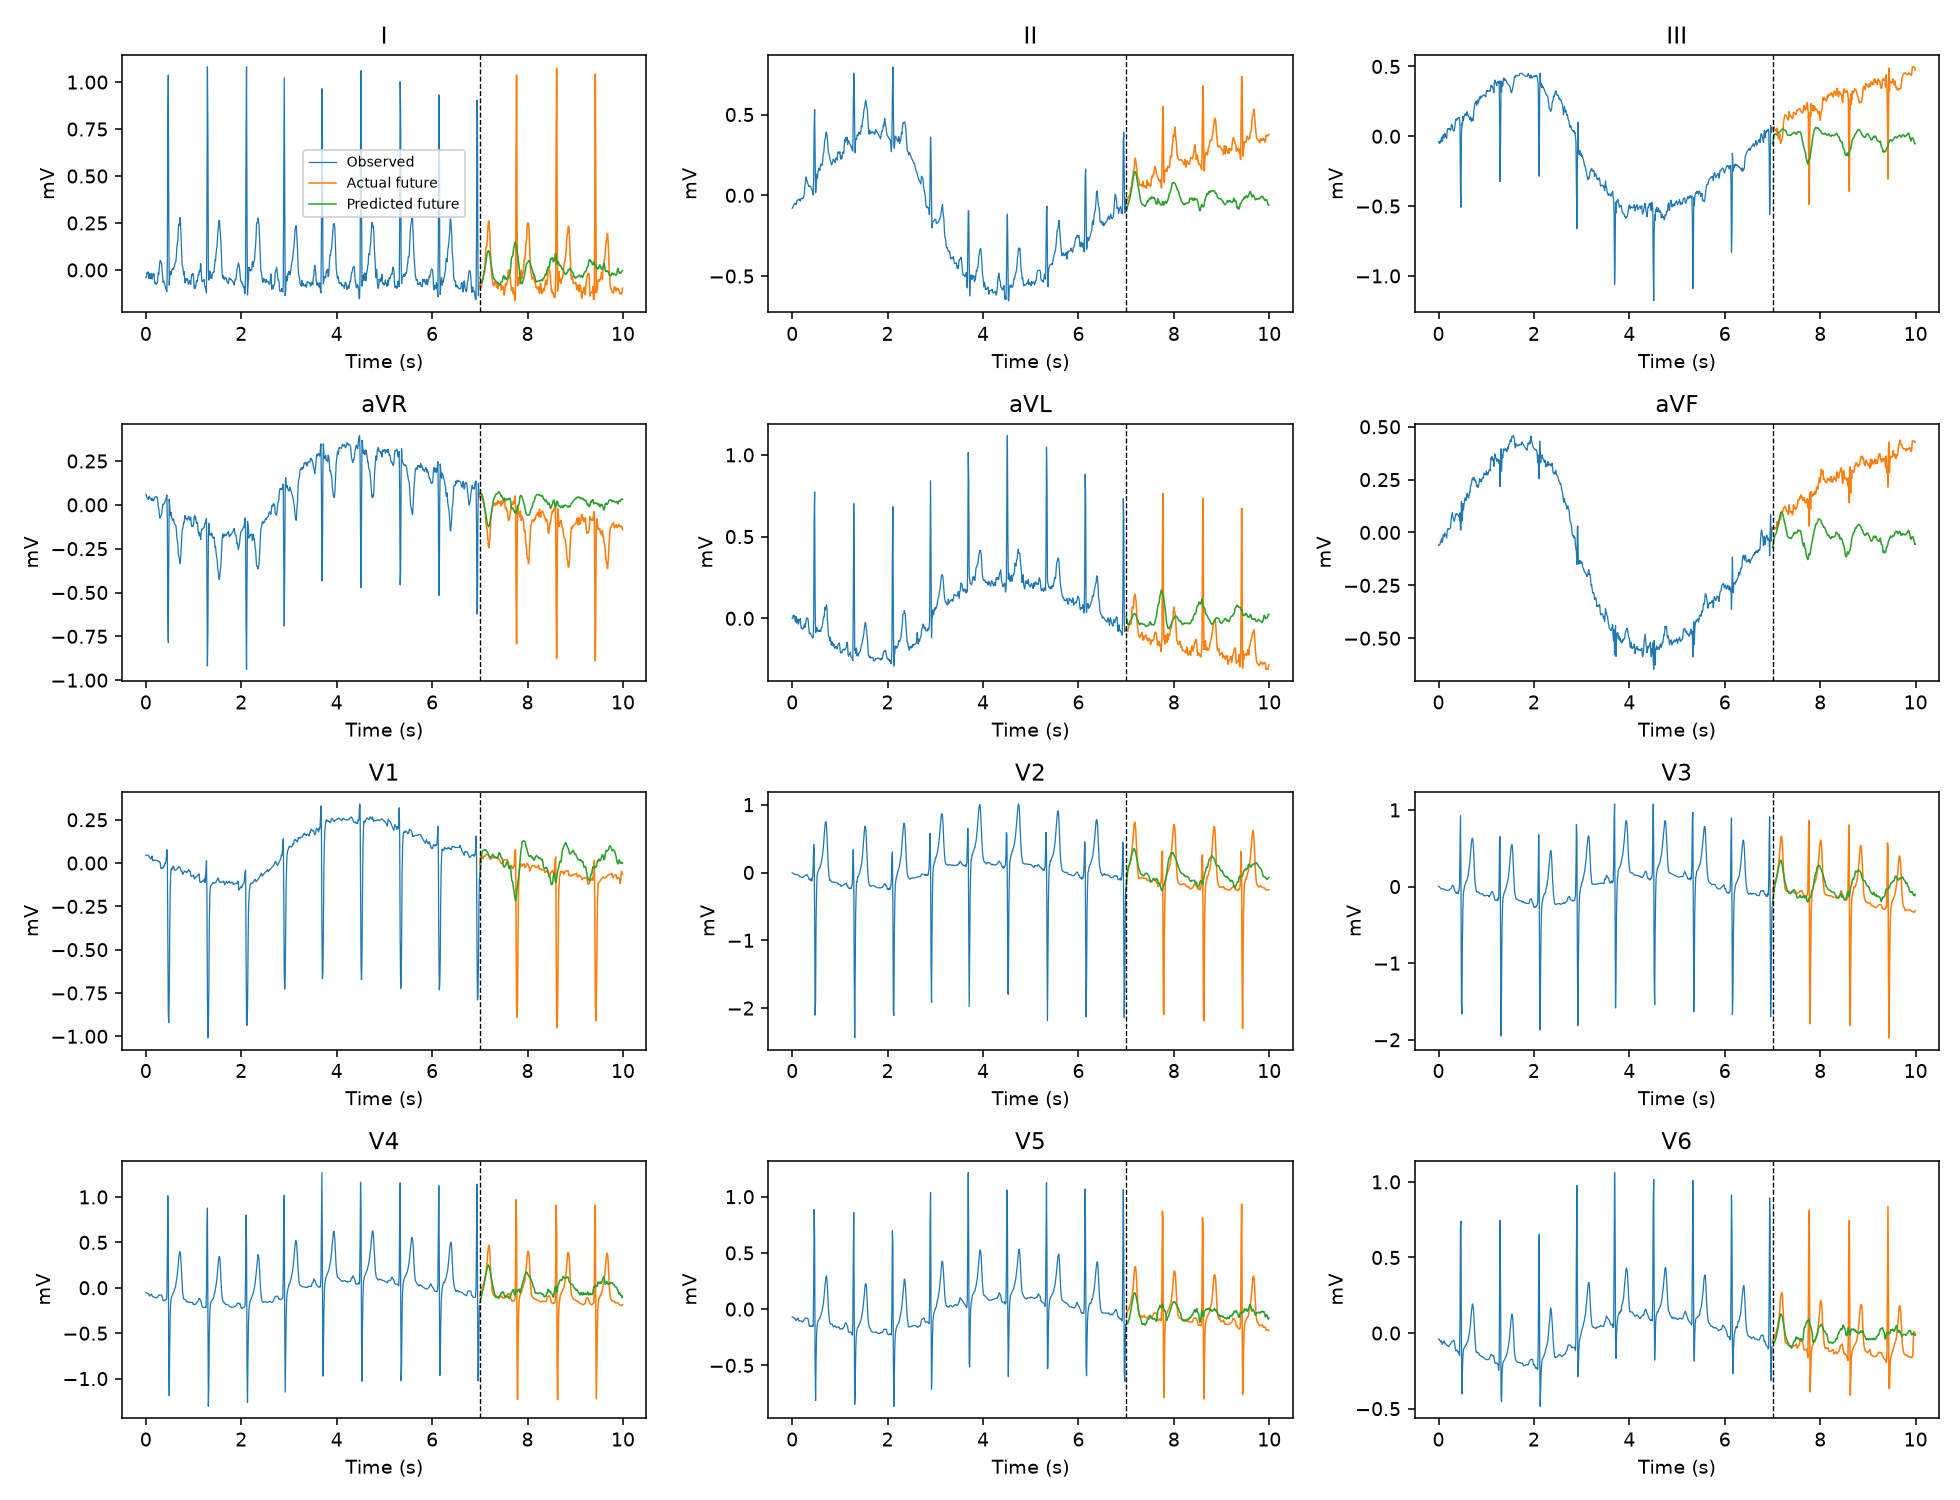
\includegraphics[width=\textwidth,height=0.78\textheight,keepaspectratio]{submission_figures/lstm.png}
\caption{LSTM: actual and predicted waveforms for each of the 12 leads, validation ECG 8.}\label{fig:lstm}
\end{figure}
\begin{figure}[p]\centering
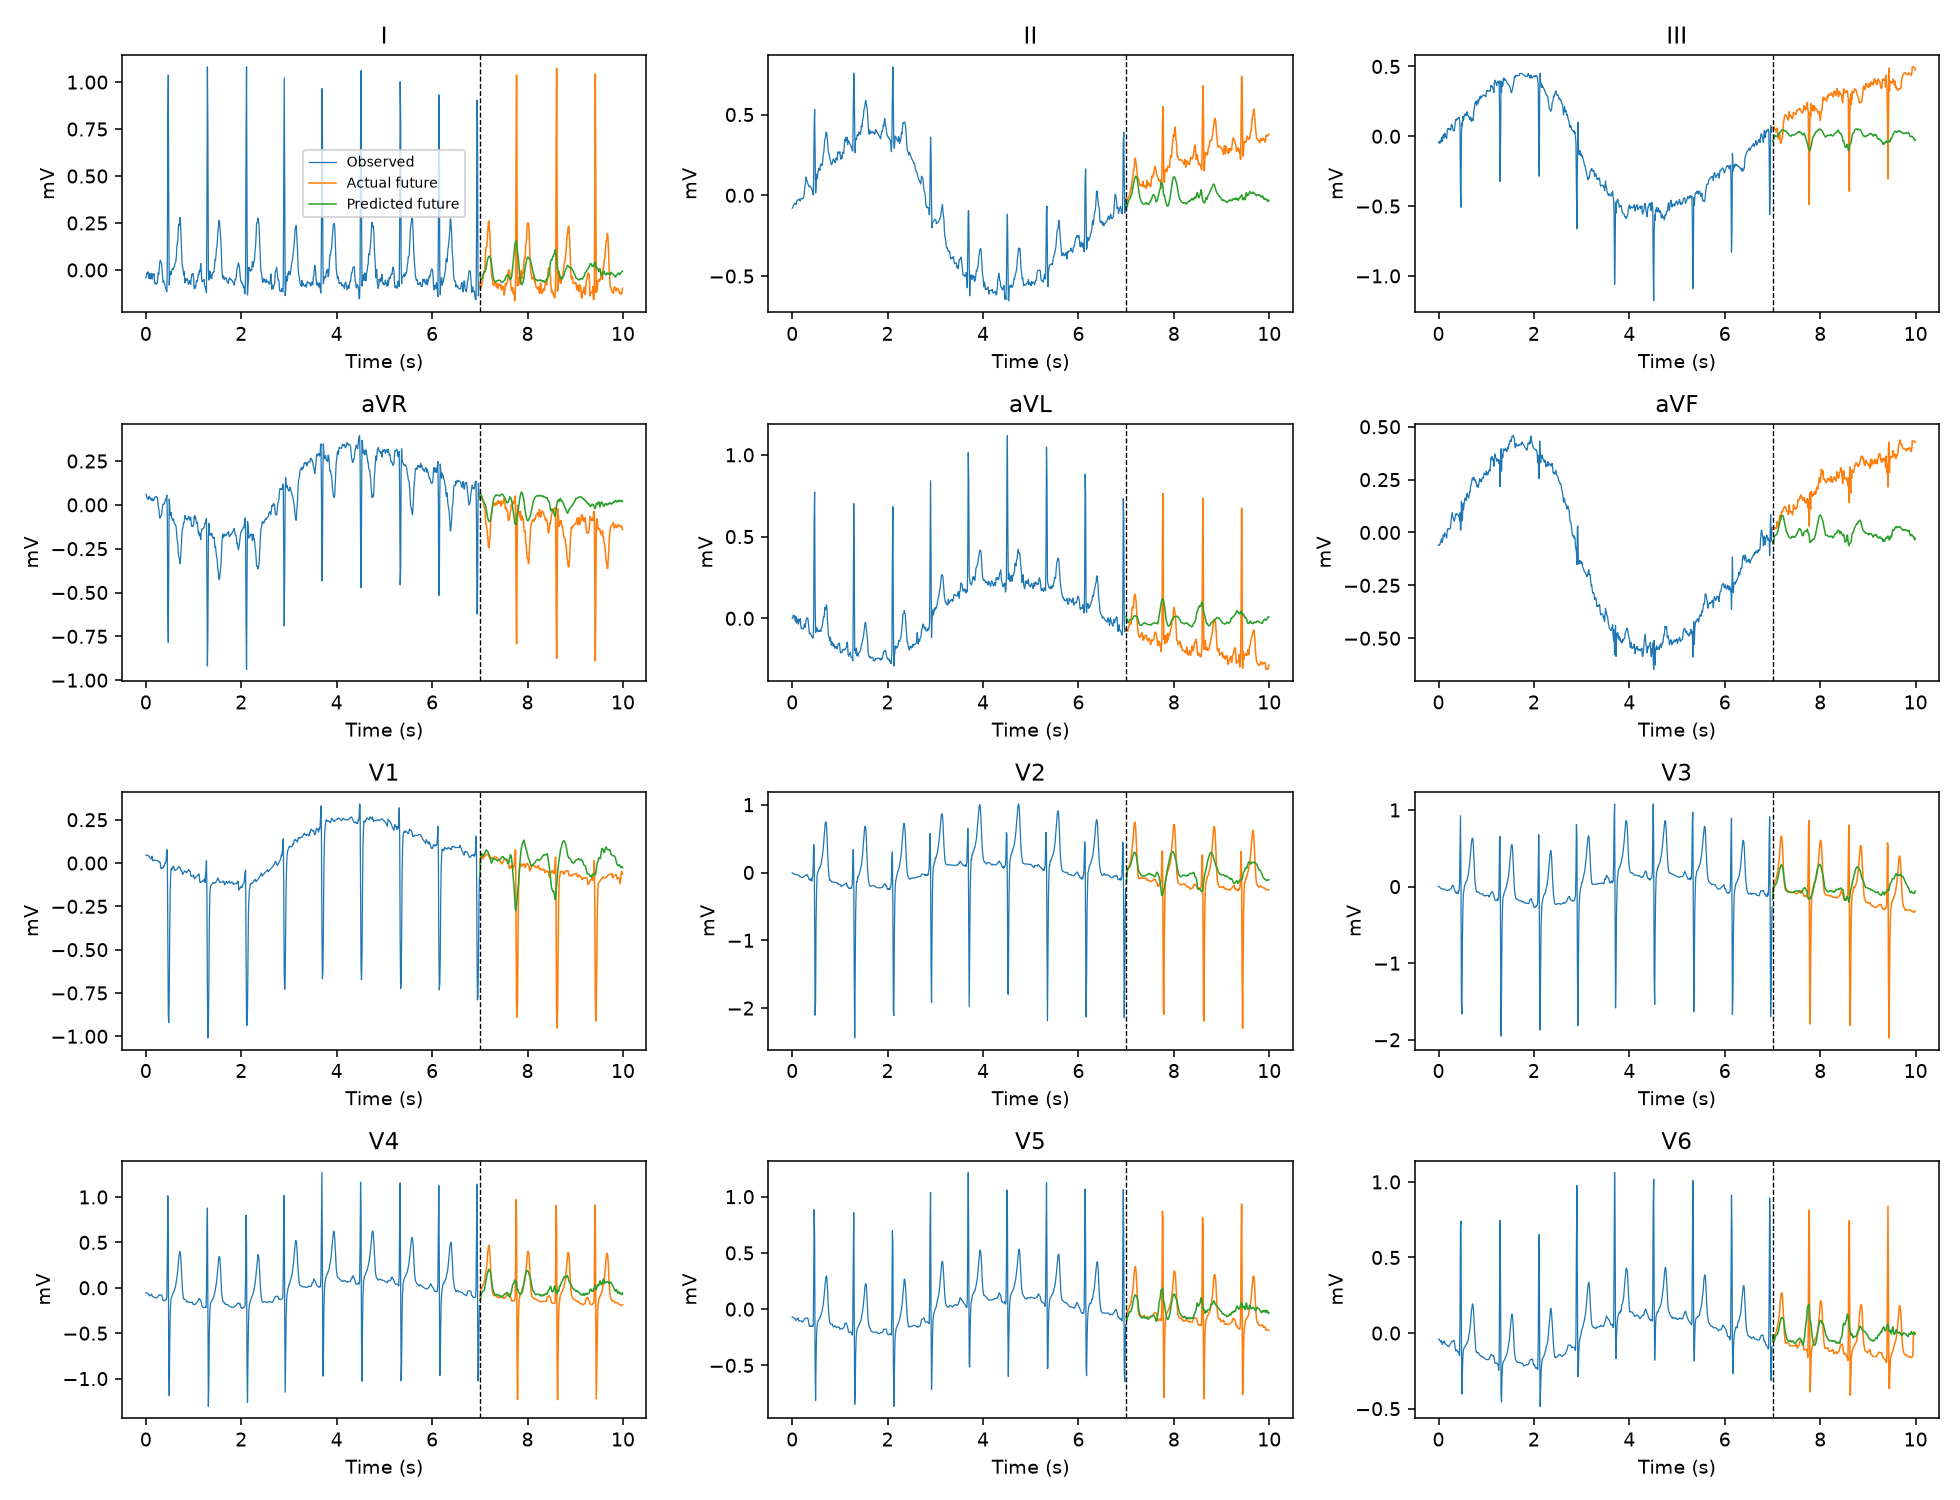
\includegraphics[width=\textwidth,height=0.78\textheight,keepaspectratio]{submission_figures/cnn.png}
\caption{CNN-LSTM: actual and predicted waveforms for each of the 12 leads, validation ECG 8.}\label{fig:cnn}
\end{figure}
\clearpage
\section{Conclusion}
Both models were implemented and evaluated on a larger training cohort for 120 epochs. CNN-LSTM obtained the lowest validation MAE and RMSE in the unfiltered setting. Filtering slightly helped the LSTM but did not improve the CNN-LSTM on these measures. The predicted-versus-actual plots show that low average error does not guarantee accurate sharp peaks. Results are limited to the validation fold and the chosen forecasting setup; the reserved test fold remains unevaluated.
\begin{thebibliography}{9}
\bibitem{ptbxl} P. Wagner et al., ``PTB-XL, a large publicly available electrocardiography dataset,'' \emph{Scientific Data}, 7, 154, 2020. Dataset version 1.0.3: \url{https://physionet.org/content/ptb-xl/1.0.3/}.
\end{thebibliography}
\end{document}
